\documentclass{article}
\title{ST3009 Weekly Questions 4}
\author{Ryan Barron // Student number: 16329561}
\date{}
\usepackage{amsmath}
\usepackage{mathtools}
\usepackage{graphicx}
\graphicspath{ {./} }
\begin{document}
\maketitle

\paragraph{Question 1}
\subparagraph{a)}
$Y=2$ corresponds to the event where the sum of the two rolled die is 2, in this case, there is only one case for that and it is (1, 1)
\subparagraph{b)}
Same idea here, except the sum is 3 and so there are only 2 events for that case, (1, 2) and (2, 1)
\subparagraph{c)}
Again, except here Y=4 and we have (2,2), (3, 1) and (1, 3)
\subparagraph{d)}
The event indicated by X is made out of 3 smaller event part of the sample space, (1, 1), (2, 2) and (3, 3). The sample space is made out of 36 total events, so the probability of $X=1$ which by definition is the probability of one of the three to occur is: $\frac{3}{36} = \frac{1}{12} = 0.0833333$

\paragraph{Question 2}
\subparagraph{a)}
X is made out of 3 coin toss and each outcome represent a $+1$ or a $-1$. Since X is calculated with 3 tosses, it can only take odd values and the minimum and maximum are $-3$ and $+3$ respectively. Other than that, it can also take the values $-1$ and $+1$ as these are the other odd values.
\subparagraph{b)}
$X=-3$ corresponds to the event of 3 tails, which has a probability of: $\frac{1}{2^3} = 0.125$
\subparagraph{c)}
$X=-1$ corresponds to the event of one extra tail, compared to the heads. With only 3 tosses, it is the probability of having 2 tails and 1 head. And there are 3 outcomes for this, namely (T, T, H), (T, H, T) and (H, T, T).
$P(X=-1) = \frac{3}{8} = 0.375$
\subparagraph{d)}
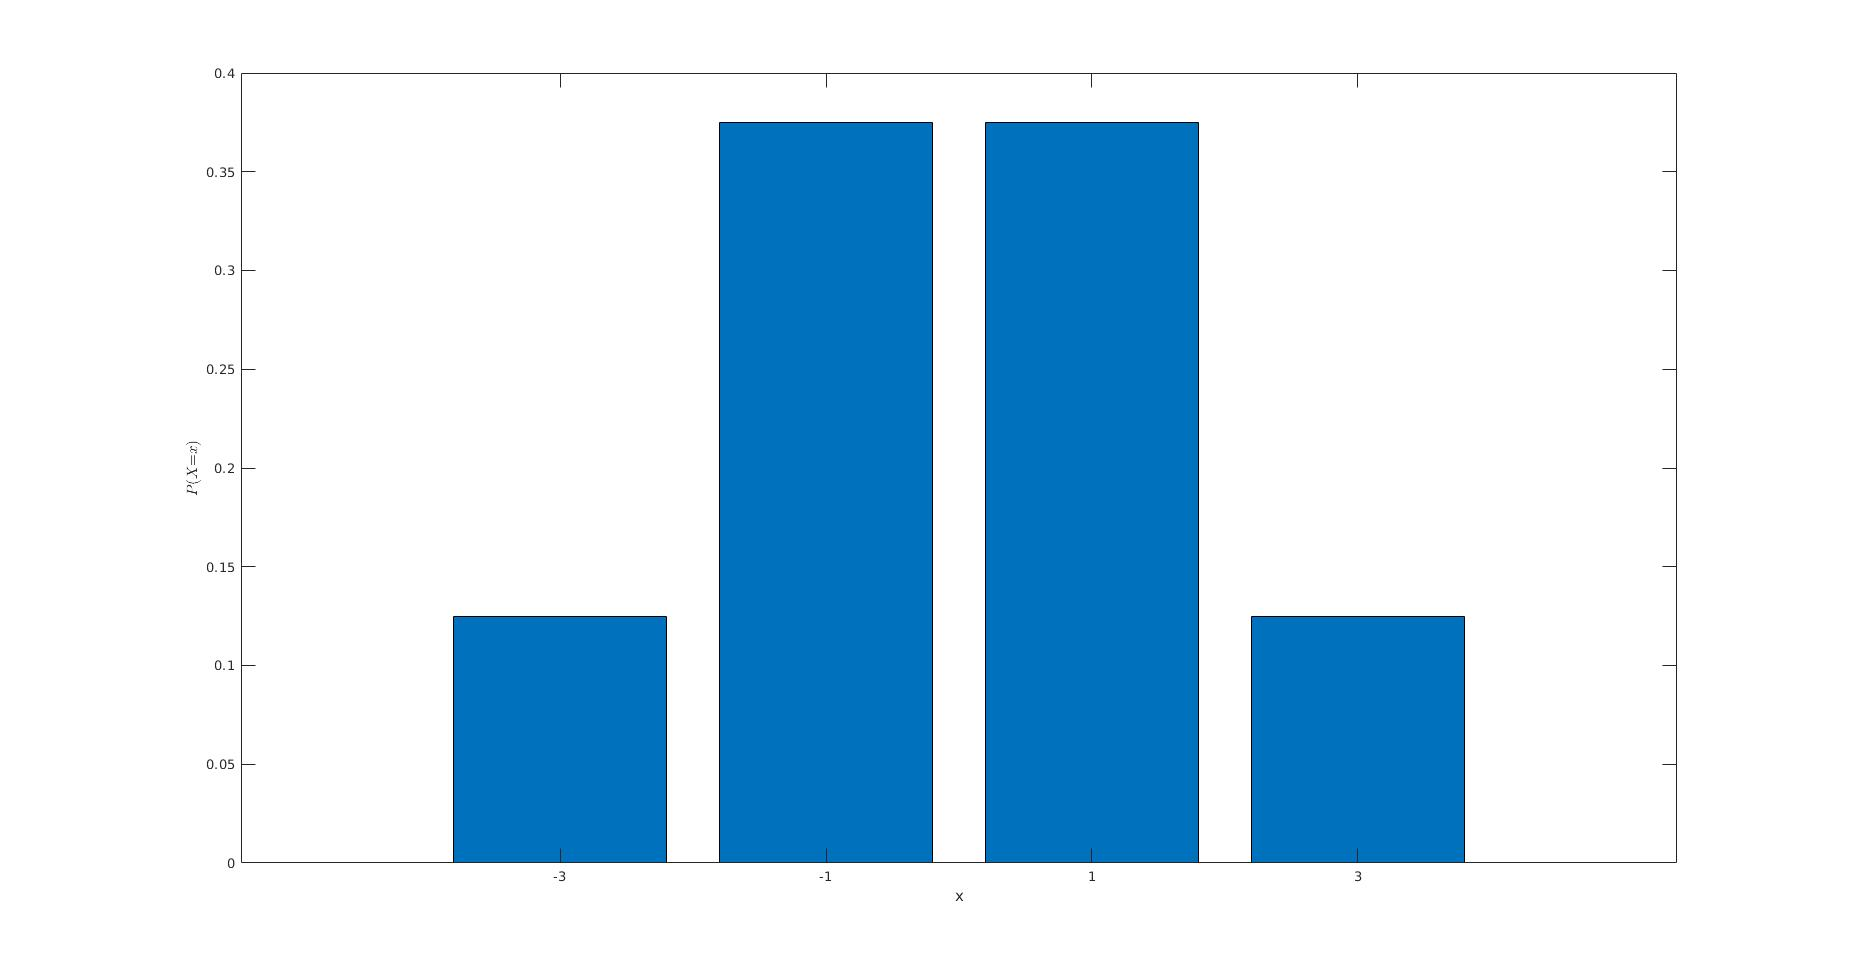
\includegraphics[width=5cm, height=5cm]{pmf.jpg}
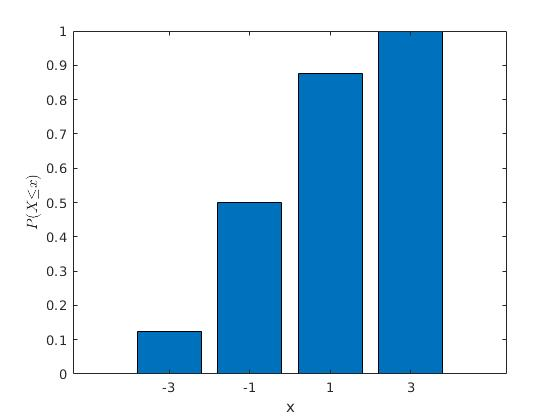
\includegraphics[width=5cm, height=5cm]{cdf.jpg}

\paragraph{Question 3}
\subparagraph{a)}
This asks "what is the probability for the minimum value to be greater or equal to 1". Well the dice can only a value between 1 and 6 inclusive. In the sample space, there are no outcome where the minimum value is below 1, that is just impossible. So $P(X\geq1) = 1$
\subparagraph{b)}
Same process here, except the minimum value has to be greater or equal to 2. This is only true when no 1 are rolled, so 
\begin{equation*}
\begin{split}
P(X\geq2) & = P(No\;1s\;rolled) \\
P(No\;1s\;rolled) & = \frac{5^4}{6^4} = 0.4822
\end{split}
\end{equation*}
\subparagraph{c)}
We need to calculate the probability P(X$\leq$k), $\forall$ k where $1\leq k\leq 6$
For each of those, it is easier to calculate the probability's complement, and subtract that from 1.
Indeed, the complement of P(X$\leq$3), for example, is the probability of P(X$>$3) which is equivalent to the probability of rolling only 4s or higher. So, we get: \\
\begin{equation*}
\begin{split}
P(X\leq1) & = 1 - P(X>1)  = 1 - \frac{5^4}{6^4}  = 0.51774691358 \\
P(X\leq2) & = 1 - P(X>2)  = 1 - \frac{4^4}{6^4}  = 0.8024691358 \\
P(X\leq3) & = 1 - P(X>3)  = 1 - \frac{3^4}{6^4} = 0.9375 \\
P(X\leq4) & = 1 - P(X>4)  = 1 - \frac{2^4}{6^4}  = 0.98765432098 \\
P(X\leq5) & = 1 - P(X>5)  = 1 - \frac{1^4}{6^4} = 0.99922839506 \\
P(X\leq6) & = 1 - P(X>6)  = 1 - \frac{0}{6^4}  = 1 
\end{split}
\end{equation*}
And so, we that, we get: \\
$
CDF(X) = \begin{cases} 0.5177, for X\leq 1 \\ 0.802, for X\leq 2 \\ 0.9375, for X\leq 3\\ 0.987, for X\leq 4\\ 0.999, for X\leq 5\\ 1, for X\leq 6\end{cases}
$
\end{document}
